%!TEX root = ../synopsis.tex

В {\bf четвёртой главе}
рассматривается методология
использования алгоритмов решения
разных классов задачи резки в существующих
CAD/CAM-системах.
Поскольку требуется обеспечить
совместную работу программного обеспечения,
разработанного в разное время разными командами разработчиков,
чрезвычайно важными становятся вопросы
организации эффективных программных интерфейсов.

Например, для хранения и обмена геометрической информацией
в САПР~<<Сириус>>
используется унаследованный двоичный формат DBS
\cite{bi:DBS},
который при значительных достоинствах
значительно затрудняет взаимодействие разных подсистем.
В рамках данной диссертационной работы
было принято решение использовать по возможности
открытые текстовые форматы для хранения и передачи данных.
В качестве основного формата был выбран формат
JavaScript Object Notation
(JSON
\autocite{bi:JSON}),
ввиду того, что
он
является стандартом де-факто во многих
современных приложениях для обмена данными,
и достаточно выразителен.

\lstinputlisting[
    language=Java,
    basicstyle=\scriptsize,
    showstringspaces=false,
    numbers=left,
    label={lst:dbs},
    captionpos=b,
    caption=JSON-файл с геометрией простейшей раскройной карты
    ]
    {media/nesting.json}

Для хранения и обмена информацией о геометрии деталей
и раскройной карты
была разработана максимально простая схема JSON,
пример такого файла для простейшей раскройной карты
приведён в Листинге~\ref{lst:dbs}.

Использование JSON
в качестве формата обмена данными
оказалось удобным на практике,
поэтому позднее были разработаны другие
форматы файлов, в частности
задания на резку и результатов резки.
Все они были формально описаны в
виде JSON-схем
\autocite*[]{bi:json-schema},
см.~\cite{bi:dbs-schema}.

Использование открытых форматов файлов позволило
также значительно упростить вопросы,
связанные с визуализацией обрабатываемой информации.
Традиционно для этого приходится
писать отдельный код,
имеющий зачастую довольно сложную структуру и решающий
множество задач, включая геометрические расчёты
и организацию пользовательского интерфейса.
В рамках данной диссертационной работы
в качестве средства визуализации
использовался экспорт в формат
Scalable Vector Graphics
(SVG),
который является стандартом де-факто,
содержит богатые возможности визуализации
и широко поддержан всеми современными браузерами.
Листинг~\ref{lst:svg}
показывает пример простейшего SVG-файла,
сгенерированного для раскройной карты,
представленной на Листинге~\ref{lst:dbs}.

\lstinputlisting[
  language=XML,
  basicstyle=\scriptsize,
  showstringspaces=false,
  numbers=left,
  label={lst:svg},
  captionpos=b,
  caption=SVG-файл для визуализации раскроя
  ]
  {media/nesting.svg}

Переход к широкому использованию SVG
позволяет также использовать зрелые современные технологии
каскадных таблиц стилей
(Cascading Style Sheets, CSS)
для управления внешним видом визуализации
(включая цвета, заливки и штриховки и анимацию)
и язык JavaScript
для добавления к визуализации
элементов интерактивности.
Один из вариантов оформления
SVG-файла из Листинга~\ref{lst:svg}
приведён на рис.~\ref{fig:nesting}.
Пользовательский интерфейс
(масштабирование и прокрутка)
обеспечивался при помощи подключения
библиотеки с открытым кодом
svg-pan-zoom
\autocite*{bi:svg-pan-zoom}.

\begin{figure}
  \centering
  \subfloat[Визуализация раскроя из Листинга~\ref{lst:dbs}]{
    \label{fig:nesting}
    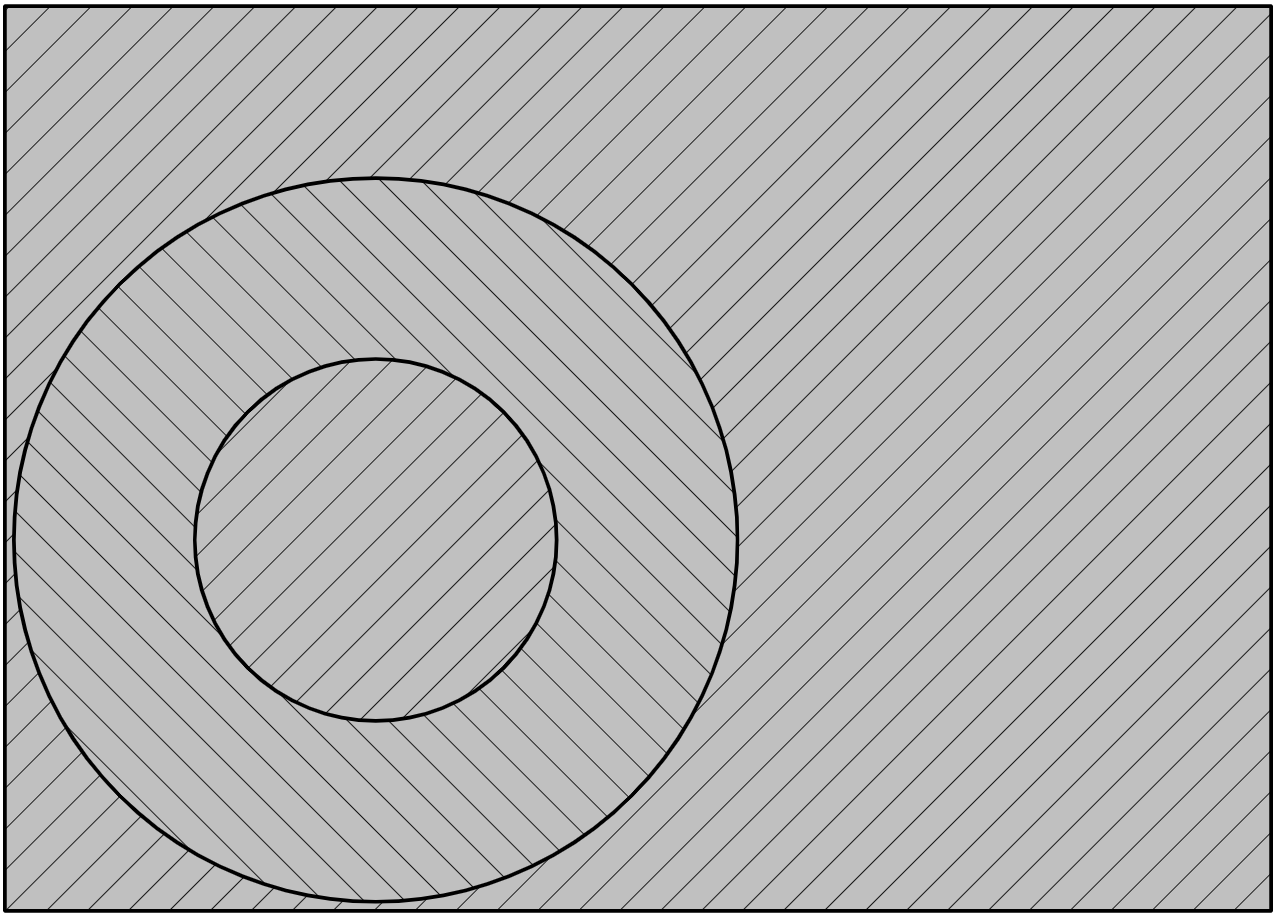
\includegraphics[width=0.4\textwidth]{nesting.png}
  }
  \subfloat[Визуализация решения задачи PCGTSP]{
    \label{fig:pcgtsp.svg}
    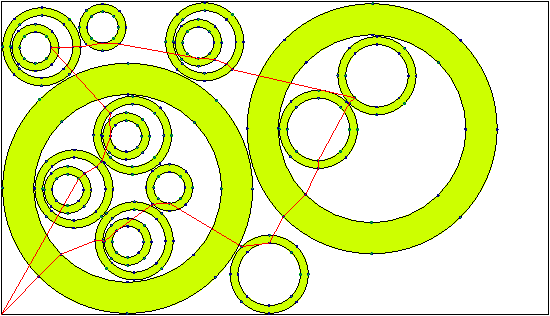
\includegraphics[width=0.5\textwidth]{34.pdf}
  }
  \caption{Примеры визуализации на основе SVG}
  \label{fig:using-svg}
\end{figure}

В ходе диссертационной работы
была разработан пакет утилит
\cite{bi:dbs2json},
обеспечивающих конвертацию между
различными форматами файлов
(включая DBS, JSON, YAML, DXF и SVG для визуализации).
Для визуализации решения задачи PCGTSP
(на основе комбинации информации,
полученной из нескольких источников),
была разработана специализированная утилита
\cite{bi:j2pcgtsp},
первоначально в форме утилиты командной строки
но позднее преобразованная
для удобства использования в
Single Page Application
(SPA).
Пример созданного ею изображения
приведён на рис.~\ref{fig:pcgtsp.svg}.
